\chapter{Theoretische Grundlagen}

\section{Aerodynamische Wirkweise des Rotors}
In der Welt der Windenergieerzeugung gibt es zwei grundlegende Bauformen von Windkraftanlagen: die Horizontalachsenwindkraftanlagen (HAWTs) und die Vertikalachsenwindkraftanlagen (VAWTs). Während Vertikalachsenanlagen bestimmte Vorteile in Bezug auf die Windrichtungsunabhängigkeit und die einfache Wartung aufweisen, haben sich Horizontalachsenwindkraftanlagen als die effizientere und weit verbreitete Option erwiesen. Diese Effizienz rührt von ihrer Fähigkeit her, höhere Energiemengen aus dem Wind zu extrahieren, insbesondere bei starken und konstanten Windverhältnissen, wie sie häufig in Offshore-Umgebungen vorkommen. Aufgrund dieser Überlegenheit in Bezug auf die Energieausbeute und die technologische Reife konzentriert sich diese Arbeit ausschließlich auf die Betrachtung und Analyse von Horizontalachsenwindkraftanlagen.

\begin{figure}[htbp] % Positionierungsoptionen: h=here, t=top, b=bottom, p=page of floats
    \centering % Zentriert das Bild
    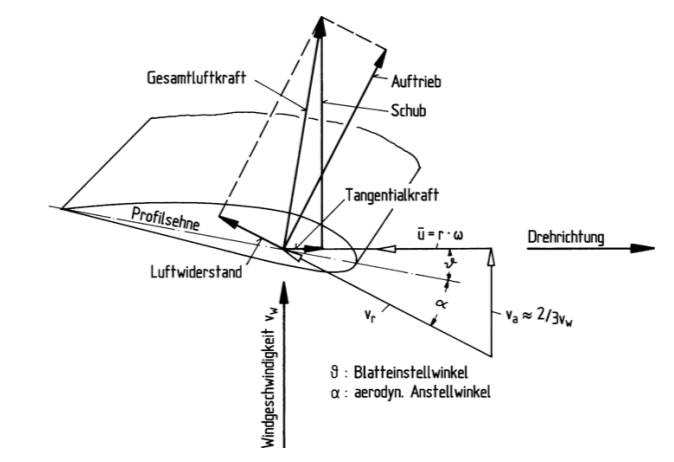
\includegraphics[width=0.8\textwidth]{figures/kraft_an_blatt.png} % Pfad zum Bild und Skalierung
    \caption{Kräfte am Rotorblatt resultieren in Drehmoment \cite{hau_physikalische_2016}, S.95} % Bildunterschrift
    \label{fig:kraft_an_blatt} % Label für Referenzen im Text
\end{figure}

Das zugrundeliegende physikalische Prinzip von HAWTs ist das gleiche wie bei Flugzeugflügeln: der Auftrieb.
Der Rotorblattquerschnitt ist so geformt, dass eine Differenz im Luftdruck zwischen der oberen und der unteren Seite des Rotorblattes entsteht, wenn Wind darüber strömt.
Die Unterseite des Rotorblattes erfährt einen höheren Druck als die Oberseite, was zu einer Auftriebskraft führt, die das Rotorblatt nach oben bzw. in Drehrichtung des Rotors zieht.
Dieser Auftrieb erzeugt um die Nabe des Rotors ein Drehmoment. Der Rotor dreht sich und treibt den Generator an.

\section{Kennzahlen}
Im Folgenden Abschnitt werden die für das Verständnis dieser Arbeit wichtigsten Kennzahlen für den Betrieb eines Rotors kurz erläutert. Für weitergehende Informationen sei auf \textcite{hau_physikalische_2016} verwiesen.
\subsection{Leistungsbeiwert von Windkraftrotoren}
Der Leistungsbeiwert \( C_P \) ist in der Aerodynamik von Horizontalachsenwindkraftanlagen (HAWAs) essentiell und quantifiziert das Verhältnis der nutzbaren mechanischen Leistung \( P \) einer Windturbine zur kinetischen Leistung des Windes \( P_{\text{wind}} \) im Rotorquerschnitt. Die Formel für \( C_P \) ist gegeben durch:

\begin{equation}
C_P = \frac{P}{\frac{1}{2} \rho A v^3}
\end{equation}

wobei \( \rho \) die Luftdichte, \( A \) die Querschnittsfläche des Rotors und \( v \) die Windgeschwindigkeit darstellt. Der Betzsche Grenzwert setzt die theoretische Obergrenze für \( C_P \) auf maximal 59,3\% fest, ausgedrückt als \( C_{P, \text{max}} = \frac{16}{27} \). Dieser Grenzwert basiert auf der Annahme, dass der Wind hinter der Turbine eine Restgeschwindigkeit behält. Real existierende Verlustquellen wie Profil- und induzierte Verluste beeinflussen die Effizienz des Rotors. Moderne Turbinendesigns zielen darauf ab, diese Verluste durch optimierte Rotorblattgeometrie zu minimieren, wobei CFD und BEM-Theorien eine entscheidende Rolle spielen.

\subsection{Schubbeiwert von Windkraftrotoren}
Der Schubbeiwert \( C_T \) ist eine weitere wichtige aerodynamische Kenngröße für Windkraftrotoren, die das Verhältnis der Schubkraft \( F_T \), die durch die Rotorblätter auf den Wind ausgeübt wird, zur kinetischen Energie des Windes im Rotorquerschnitt darstellt. Mathematisch lässt sich \( C_T \) definieren als:

\begin{equation}
C_T = \frac{F_T}{\frac{1}{2} \rho A v^2}
\end{equation}

wobei \( F_T \) die Schubkraft ist. Ein hoher Schubbeiwert kann auf eine effektive Energieübertragung hinweisen, führt jedoch auch zu erhöhten mechanischen Belastungen der Turbinenstruktur. Die Auslegung zielt daher auf ein optimales Gleichgewicht zwischen Energieextraktion und struktureller Belastung ab. Im Kontext der Multirotor-Winkraftanlagen kommt dem Schubbeiwert eine weitere Bedeutung zu. Kontrollierte Schubkraftunterschiede zwischen den einzelnen Rotoren könnten für die Ausrichtung der gesamten Anlage entsprechend der Windrichtung genutzt werden. 

\subsection{Schnellaufzahl}
Die Schnellaufzahl \( \lambda \) ist ein maßgeblicher Parameter in der Aerodynamik von Windenergieanlagen. Sie berechnet sich aus dem Verhältnis der Umfangsgeschwindigkeit der Rotorblattspitze \( u \) zur Windgeschwindigkeit \( v \) an der Turbine:

\begin{equation}
\lambda = \frac{u}{v}
\end{equation}

Sowohl Leistungs- als auch Schubbeiwert des Rotors hängen von der Schnelllaufzahl ab. Im Betrieb sollte die Drehzahl des Rotors so geregelt werden, dass die optimale Schnelllaufzahl erreicht wird. Der genaue Wert der Optimalen Schnelllauf hängt vor Allem von der Anzahl der Rotorblätter und deren Design ab. Im Entwurfsprozess werden die Rotorblätter auf eine bestimmte Entwurfsschnelllaufzahl hin optimiert.

\section{Aerodynamik eines Rotorblattes}
\subsection{Grundbegriffe}
Aerodynamische Profile unterliegen Konventionen zur Beschreibung ihrer Formgebung. Die wichtigsten Begrifflichkeiten werden in \ref{fig:profil_begriffe} dargestellt.

\begin{figure}[htbp] % Positionierungsoptionen: h=here, t=top, b=bottom, p=page of floats
    \centering % Zentriert das Bild
    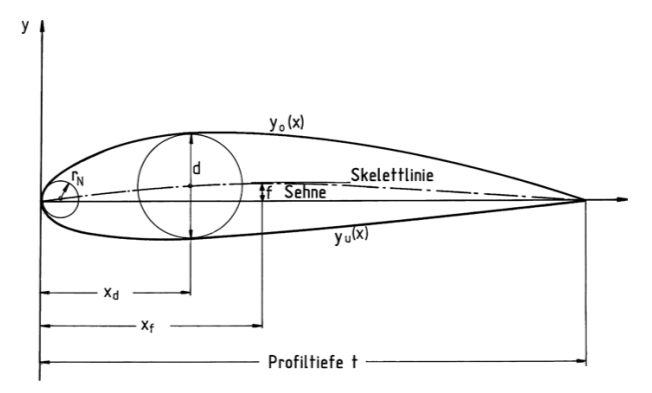
\includegraphics[width=0.8\textwidth]{figures/profil_begriffe.png} % Pfad zum Bild und Skalierung
    \caption{Grundbegriffe bei aerodynamischen Profilen \cite{hau_physikalische_2016}, S.130, modifiziert} % Bildunterschrift
    \label{fig:profil_begriffe} % Label für Referenzen im Text
\end{figure}

\begin{itemize}
    \item Profiltiefe \( c \) (Länge der Sehne)
    \item Maximale Wölbung \( f \)
    \item Wölbungsrücklage \( x_f \)
    \item Maximale Profildicke \( d \), als Durchmesser des größten Kreises auf der Skelettlinie
    \item Dickenrücklage \( x_d \)
    \item Nasenradius \( r_N \)
    \item Profilkoordinaten \( y_o(x) \) und \( y_u(x) \) der Ober- bzw. Unterseite
\end{itemize}

\subsection{Kräfte und Kennzahlen}

In der Aerodynamik, insbesondere bei der Betrachtung von Windkraftrotorblättern, sind die Auftriebs- und Widerstandskräfte zentral. Diese Kräfte werden jedoch nicht direkt verwendet, sondern durch dimensionslose Beiwerte dargestellt. Der Grund dafür liegt in der universellen Anwendbarkeit und Vergleichbarkeit dieser Beiwerte.

Der Auftriebsbeiwert \( c_l \) und der Widerstandsbeiwert \( c_d \) ermöglichen es, die Leistung eines Profils unabhängig von seiner Größe oder den spezifischen Flugbedingungen zu bewerten. Der Auftriebsbeiwert \( c_l \) ist definiert als:

\begin{equation}
c_l = \frac{L}{\frac{1}{2} \rho v^2 c}
\end{equation}

wobei \( L \) die Auftriebskraft, \( \rho \) die Luftdichte, \( v \) die Strömungsgeschwindigkeit und \( c \) die Sehnenlänge des Profils ist. Der Widerstandsbeiwert \( c_d \) wird ähnlich berechnet:

\begin{equation}
c_d = \frac{D}{\frac{1}{2} \rho v^2 c}
\end{equation}

Die Gleitzahl, die die aerodynamische Effizienz des Profils angibt, wird als das Verhältnis von Auftrieb- zu Widerstandsbeiwert definiert:

\begin{equation}
E = \frac{c_l}{c_d}
\end{equation}

Eine hohe Gleitzahl bedeutet, dass das Profil effizient Auftrieb erzeugt, während der Widerstand gering bleibt. 
Bei Windkraftrotoren ist eine hohe Gleitzahl wichtig, da sie direkt die Menge an nutzbarer Energie beeinflusst, die aus dem Wind extrahiert werden kann. Die Optimierung des Profils zielt daher im Allgemeinen darauf ab, eine möglichst hohe Gleitzahl zu erreichen, um die Effizienz und Leistung der Windturbine zu maximieren.


\section{Methoden der Rotorblattauslegung}
\subsection{Auslegung nach Betz und Schmitz}
\label{subsec:betz-schmitz-auslegung}
Historisch betrachtet basiert die Theorie der Rotorblattauslegung auf den grundlegenden Arbeiten von Albert Betz und Hermann Schmitz, die Anfang des 20. Jahrhunderts die Grenzen und Möglichkeiten der Windenergienutzung untersuchten. Betz legte mit seinen Theorien den Grundstein und lieferte Beziehungen für die optimale Flügeltiefenverteilung \( c(r) \) sowie die Blattverwindung \( \vartheta(r) \).Seine Theorie geht allerdings davon aus, dass sich die Lustströmung nach dem Rotor lediglich verlangsamt, aber nicht in seiner Richtung abgelenkt wird. Verluste durch den induzierten Widerstand bzw. Blattspitzenverluste sowie Profilwiderstand und Drallverluste vernachlässigt er. Schmitz erweiterte später diese Theorie, indem er zusätzliche Verluste in Betracht zog und so die Auslegung von Rotorblättern weiter verfeinerte. 

Die Flügeltiefe  und die Verwindung  eines Rotorblattes sind zwei entscheidende geometrische Parameter, die die aerodynamische Leistung und die Effizienz eines Windkraftrotors bestimmen. Sie lassen sich aus den folgenden Formeln ableiten:

\begin{equation}
c_{\text{opt,Schmitz}} = \frac{16 \pi}{z \cdot c_A} \cdot r \cdot \sin^2 \left( \frac{1}{3} \arctan \left( \frac{1}{\lambda_A }\frac{R}{r} \right) \right)
\end{equation}

\begin{equation}
\vartheta_{\text{opt,Schmitz}}(r) = \frac{2}{3} \arctan \left( \frac{1}{\lambda_A} \frac{R}{r} \right) - \alpha \left( \varepsilon_{\text{max}}, r \right)
\end{equation}



wobei \( r \) der lokale Radius entlang der Rotorblattspannweite ist, \( z \) die Anzahl der Rotorblätter, \( B \) der Blattkorrekturfaktor, \( R \) der Rotorradius, \( \lambda \) die Schnellaufzahl, \( \lambda_{opt,Betz} \) die optimale Schnellaufzahl nach Betz, \( \phi(r) \) der lokale Strömungswinkel und \( \alpha(r) \) der Anstellwinkel des Profils. Der Parameter \( \Gamma \) steht für das Verhältnis von Auftrieb zu Widerstand.

Die korrekte Auslegung von \( c(r) \) und \( \theta(r) \) ist entscheidend für die Leistungsfähigkeit des Rotors. Die Flügeltiefe muss so dimensioniert sein, dass sie die Kräfte über die gesamte Länge des Blattes optimal verteilt, während die Verwindung sicherstellt, dass die Anstellwinkel über den Radius hinweg die aerodynamische Effizienz maximieren. Die hier beschriebenen Formeln sind idealisiert und müssen in der Praxis durch iterative Verfahren und CFD-Simulationen verifiziert und angepasst werden.

\subsection{Simulation mit Blatt-Element-Methode (BEM}
\section{Besonderheiten sehr kleiner Windkraftanlagen}